\section{PSoC Master implementering} \label{sec:PSoC_Master_impl}

Dette afsnit omhandler overvejelser og det udførte design for PSoC Master blokken i systemet.

\begin{figure}[h]
\centering
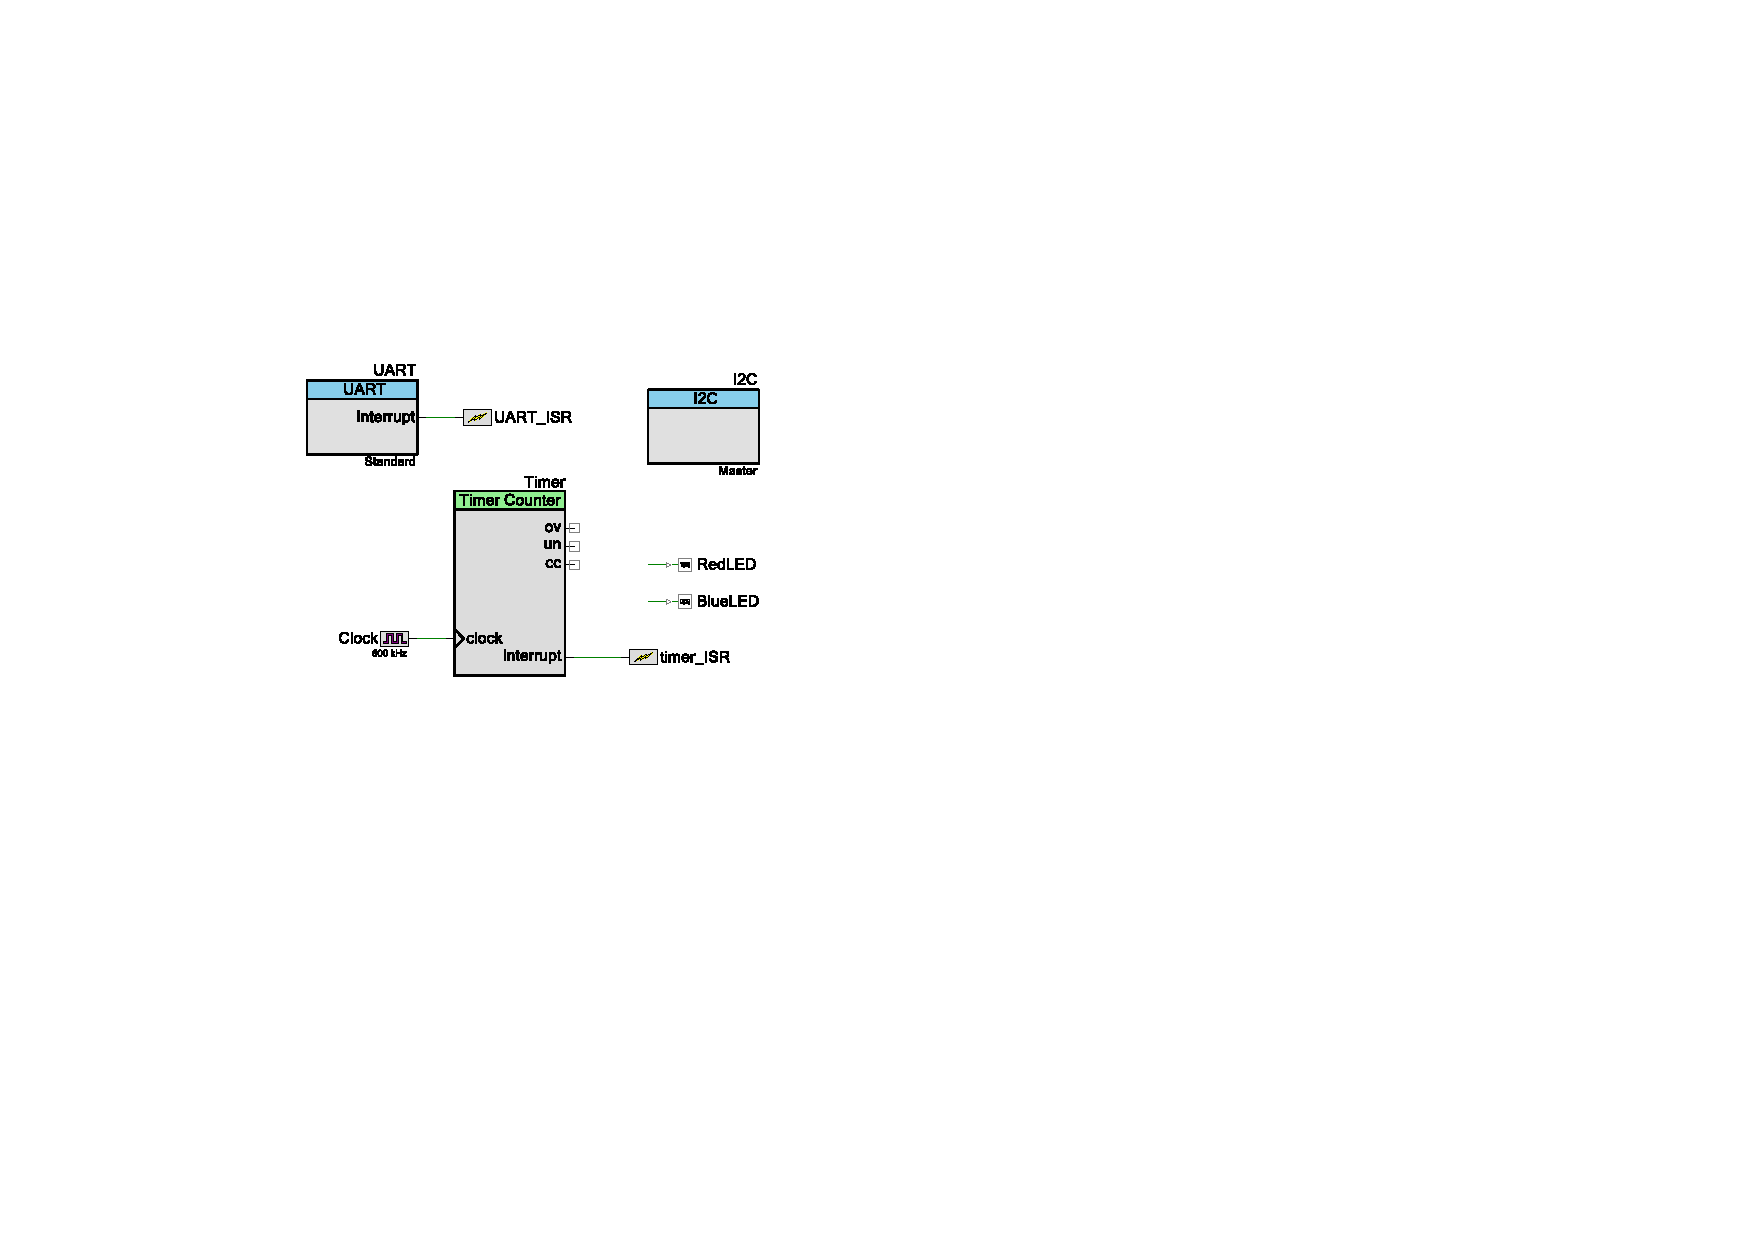
\includegraphics[width=\textwidth*3/5, trim=145 270 475 170, clip=true]{../fig/TopDesign_PSoC_Master}
\label{fig:psoc_master_topdesign}
\caption{TopDesign.cysch for PSoC\_Master}
\end{figure}

I Figur \ref{fig:psoc_master_topdesign} ses topdesignet for PSoC Master. Ud fra dette ses det at vi overordnet set har at gøre med en UART, som genererer interrupts, en Timer, som genererer interrupts, en I2C blok og to outputs til LED. 
Selve topdesignet er lavet ud fra de behov der er stillet i Design-fasen. Der blev under implementeringen af UART overvejet brug af en anden UART komponent, men problemet viste sig at ligge i et tidligere design-valg angående paritet.

\clearpage

\subsection{\IIC implementering}
I forbindelse med implementeringen af \IIC klassen blev prototyperne oprettet jf. \IIC protokollen (se side REFREFREF. 
Klassen reagerer på kald fra timer interruptet, og er i stand til at sende og indhente information hhv. til og fra sensorer og aktuatorer der er tilkoblet \IIC-bussen. 
Det blev valgt fra start af, at det mest ideelle når der skal sendes data, er at der altid er noget data klar til at blive sendt. 
Pga. dette er der behov for at timer interrupten kan kalde \IIC-klassens metoder og derved opdatere de værdier der skal indhentes til DSP klassen. Pga. problemer med de bestilte sensorer, er temperatursensoren LM75 blevet anvendt istedet for den tidligere oplyste temperatur/luftfugtsensor. Ligeledes er lyssensorens implementering nedprioriteret, pga. tidsmangel. 

\begin{lstlisting}[language=C,caption=Implementering af getTemp(),label=lst:I2C_Class_getTemp()]
int8 getTemp(int32* temp){

    uint8 dataget[2] = {0,0};
    uint32 errorStatus[2] = {9,9};      // For debugging and error handling
    
    I2C_I2CMasterClearReadBuf();
    errorStatus[0] = I2C_I2CMasterSendStart(TEMP_SENSOR_ADDRESS, I2C_I2C_READ_XFER_MODE);
    if (errorStatus[0] == I2C_I2C_MSTR_NO_ERROR){
        dataget[0] = I2C_I2CMasterReadByte(I2C_I2C_ACK_DATA);
        dataget[1] = I2C_I2CMasterReadByte(I2C_I2C_NAK_DATA);
        errorStatus[1] = I2C_I2CMasterSendStop();
    }
    else{
        I2C_I2CMasterSendStop();
        return -1;
    }
...
\end{lstlisting}

I Figur \ref{lst:I2C_Class_getTemp()}, ses der et eksempel på håndtering af en request fra timer interruptet. 
Som det kan ses, bliver der kaldt nogle metoder der kommunikerer med slaven over bussen. For at LM75 reagerer på masterens kald, sendes der en slaveadresse og en read-request. Herefter sender slaven to bytes, som gemmes i bufferen og til sidst bliver der sendt en stopsekvens. Jf. \IIC protokollen på side \pageref{sec:I2C_protokol}, indeholder de to bytes temperaturdata, hvor MSB angiver om temperaturen er negativ eller ej (værdien er signed) og de 8 efterfølgende bits angiver selve temperaturen med en halv grads opløsning. 

Fra aktuatorens side er det valgt, at når der modtages en kommando over \IIC, aktiveres der en interrupt der holder håndterer den pågældende kommando. For \IIC-klassen betyder det at uanset tidspunktet, kan der sendes kommandoer hele tiden, men af hensyn til svaret der skal modtages over bussen, holder masteren klokken lav, indtil enten et svar eller en fejl er modtaget. Princippet i read/write funktionen er, at masteren blokerer for andre interrupts og sender en slaveadresse ud på bussen, hvorefter der kommer et acknowledge tilbage fra slaven, som derefter sender et antal bytes ud. Det samme kan overordnet siges om write metoden. Eftersom \IIC er lavet som master/slave forhold som standard vil det, medmindre der er tale om et multimaster system, altid være masteren der dominerer bussen, således må slaven aldrig holde clocken LOW. 

\begin{lstlisting}[language=C,caption=Implementering af getActuatorStatus(),label=lst:I2C_Class_getActuatorStatus()]
int8 getActuatorStatus(uint8* window, uint8* heat, uint8* vent, uint8* irrigation){
    uint8 result = 0;
    int RDbuf = 2;
    uint8 dataget[RDbuf];
    
    //I2C_I2CMasterClearStatus();     // Clear status flags TODO test
    
    while (0u == (I2C_I2CMasterStatus() & I2C_I2C_MSTAT_WR_CMPLT)); //Wait for the bus to be ready
    
    CyDelay(60);
    
    I2C_I2CMasterClearReadBuf();
    result = I2C_I2CMasterReadBuf(ACTUATOR_ADRESS, dataget, RDbuf, I2C_I2C_MODE_COMPLETE_XFER);
    
    while (0u == (I2C_I2CMasterStatus() & I2C_I2C_MSTAT_RD_CMPLT)); //Wait for the dataget array to be updated
\end{lstlisting}

Det kan ses på Listing \ref{lst:I2C_Class_getActuatorStatus()} linje 8 og 15, at systemet venter på, at bussen bliver ledig. Under debugging af \IIC-klassen var der store problemer, netop med at bussen ikke var ledig under fx. en læsning. Problemet viste sig at ligge i rækkefølgen PSoC4 afvikler de interrupts der kommer. Eftersom standard prioritering af interrupts sætter første interrupt kald (UART) som højst prioriteret, venter systemet med at udføre alle andre metodekald indtil efter UART'en har fået et returkald. Dog udførte systemet stadig en del af funktionaliteten for read/write \IIC, hvilket betød at bussen var optaget i den tid der blev forsøgt at læse. Løsningen på problemet viste sig at være en genopbygning af UART-interruptet, således alt funktionelt blev rykket ud i main og at der bliver sat flag, når det er nødvendigt.

\begin{lstlisting}[language=C,caption=Implementering af getActuatorStatus(),label=lst:I2C_Class_getActuatorStatus()]
...
if ((result == I2C_I2C_MSTR_NO_ERROR) && (I2C_I2CMasterGetReadBufSize() != 0)){
	if (window){                                   			// Expecting to receive MSB first 
    	*window = (dataget[0] >> 4);      					// Shifting out the 4 LSB.
        #ifdef debugging
        	UART_UartPutChar(*window+48);
        #endif
	}
...
\end{lstlisting}



\subsection{UART implementering}
UART klassen har til formål at modtage kommandoer fra DevKit8000, tolke disse og give passende svar. 

Generelt set er klassen implementering med udgangspunkt i vores UART protokol, men er udvidet således at der let kan implementeres flere trin i hhv. kontrol af vindue, motor og vanding. UART klassen gør brug af UART komponenten (SCB) vist i Figur \ref{fig:psoc_master_topdesign}.

\begin{lstlisting}[language=C,caption=Implementering af respondTemp(),label=lst:psoc_master_respondTemp]
int8 respondTemp(uint8 temp){
    if(temp){
        // If temp is between 1 and 200(both inclusive) "T" and temp is sent to DevKit8000
        UART_UartPutChar('T');
        UART_UartPutChar(temp);
        return 0;
    }
    else{
        // If temp isn't between 1 and 200(both inclusive) "XT" is sent to DevKit8000
        UART_UartPutChar('X');
        UART_UartPutChar('T');
        return -1;
    }
}
\end{lstlisting}

I Listing \ref{lst:psoc_master_respondTemp} vises et eksempel på en af funktionerne der håndterer svar via UART. De øvrige funktioner i klassen fungerer på samme måde. Funktionen modtager den værdi, der skal sendes tilbage til DevKit8000. Hvis parametren er 0 vil det sige at der er sket en fejl. Når funktionen kaldes kaldes den med returværdi fra DSP klassen, som beskrevet i afsnit \ref{sec:DSP_impl}.

\begin{lstlisting}[language=C, caption=Implementering af dkRequest(), label=lst:psoc_master_dkreq]
uint8 dkRequest(void){
    // Reads the UART buffer
    return UART_UartGetChar();
}
\end{lstlisting}

Vi har ydermere valgt at indkapsle læsningen fra UART ved hjælp af dkRequest() funktionen vist i Listing \ref{lst:psoc_master_dkreq}. 
Grunden til at vi har valgt at implementere denne er for at sikre os at hvis UART protokollen skulle ændre sig i fremtiden, kan disse ændringer tages højde for i denne funktion inden PSoC Master controllerklassen skal håndtere input fra UART.

\subsection{DSP implementering}\label{sec:DSP_impl}
DSP klassen agerer både digital signal processor og domæneklasse for vores måledata. 
Hver type af data er gemt i sit eget array, som vist i Listing \ref{lst:DSP_decl}. 
Hvert arrays har ligeledes en pointer til den næste plads i arrayet der skal overskrives.

\begin{lstlisting}[language=C, label=lst:DSP_decl, caption=Deklaration af arrays og pointers]
// Private data members
int32 tempArray[ARRAYSIZE];
int32* tempArrayPtr;
int32 humArray[ARRAYSIZE];
int32* humArrayPtr;
int16 soilHumArray[NBR_OF_SOILHUM_SENSORS][ARRAYSIZE];
int16* soilHumPtr[NBR_OF_SOILHUM_SENSORS];
int32 lightArray[ARRAYSIZE];
int32* lightArrayPtr;
uint8 temp, hum, soilHum[NBR_OF_SOILHUM_SENSORS], light;     // Used for storing the newest value
\end{lstlisting}

Arrays'ne bliver brugt til at gemme en række datapunkter i råt format. Disse data punkter kan herefter konverteres og midles.
For jordfugt (soilHumArray), er der oprettet et todimensionelt array således at der kan gemmes et array med data for hver af de 6 sensorer.

Når der er målt en ny værdi fra en sensor, via \IIC klassen, bliver den indlæst i DSP klassen med input-funktionerne.

\begin{lstlisting}[language=C, label=lst:DSP_inputTemp, caption=Funktion til at indlæse en sensorværdi i DSP klassen]
void inputTemp(int32* temp){
    *tempArrayPtr = *temp;      // The input value is written to the array
    tempArrayPtr++;             // The pointer is moved to the next place in array
    if(tempArrayPtr > &tempArray[ARRAYSIZE-1]){
        tempArrayPtr = &tempArray[0];   // If the pointer is pointing past the end of the array it's reset
    }
    
    avgTemp();      // The average value is calculated and onverted into temp(globel) 
}
\end{lstlisting}

I Listing \ref{lst:DSP_inputTemp} ses inputTemp funktionen der indlæser den målte værdi i tempArray vha den tilhørende pointer tempArrayPtr. Pointeren flyttes herefter til næste plads i arrayet. Arrayet overskrives på ny når dette er fuldt. Til sidst kaldes den private funktion avgTemp.

\begin{lstlisting}[language=C, label=lst:DSP_avgTemp, caption=Funktion til at indlæse en sensorværdi i DSP klassen]
void avgTemp(void){
    uint8 skip = 0;
    int64 total = 0;
    {
        uint8 i;
        for(i = 0 ; i<ARRAYSIZE ; i++){
            if(tempArray[i]>=0){
                total += tempArray[i];
            }
            else{
                skip++;
            }
        }
    }
    // Makes sure that enough datapoints are pressent
    if(ARRAYSIZE-skip>=NMR_OF_VALID_DATAPOINTS_NEEDED){    
        int32 avg = total/(ARRAYSIZE-skip);		// Calculate the average value
        
        // TODO limit temp output to 1 and 200
        
        temp = (uint8)avg;
    }
    else{
        temp = 0;
    }
}
\end{lstlisting}
%TODO latlisting indhold skal opdateres

I Listing \ref{lst:DSP_avgTemp} vises avgTemp funktionen. Denne har flere funktoner, da den kun skal sørge for at der er nok datapunkter til at midle arrayet.
%TODO Skal laves færdig

\subsection{Controller implementering}

PSoC\_Master controller-klassen er som udgangspunkt designet ud fra at blive styret af hvilke kommandoer der er modtaget på UART'en. På den måde agerer vores 'master' slave for DevKit8000. 
For at huske den nuværende status er der oprettet en \texttt{enum} med den nuværende status samt ekstra buffer til at holde styr på hvilken vandingsaktuator der modtages data omkring.

\begin{lstlisting}[language=C, label=lst:PSoC_m_dec, caption=Deklaration af buffers og flag.]
// Buffers / flags
typedef enum {IDLE, ADJW, ADJH, ADJV, ADJI} state;
volatile state theState = IDLE;
volatile int8 irrigationIndex = 0;
uint8 newByte = 0;
uint8 buff;
\end{lstlisting}

Ydermere er der lavet en form for debugging ved hjælp af de tre farvede LED'er på PSoC4 Pioneer Kit. Der tændes fx for den røde LED når et interrupt sker på timeren og for den blå når et interrupt sker på UARTen.

Når der sker et interrupt på UART'en, sættes flaget \texttt{newByte} til 1 og der fyldes data i bufferen. Dette ses i Listing \ref{lst:PSoC_m_uart_int}.

\begin{lstlisting}[language=C, label=lst:PSoC_m_uart_int, caption=ISR for UART.]
// UART ISR
CY_ISR(UART_ISR){
    newByte = 1;
    buff = dkRequest();
    UART_ClearRxInterruptSource(UART_GetRxInterruptSourceMasked());     // Clear interrupt flag
}
\end{lstlisting}

Årsagen til at vi har valgt at sætte et flag er at vi hurtigst muligt vil ud af interrupt service rutinen samt at det gav os problemer at have al funktionaliteten som kald fra UART ISR.

Der er herefter udarbejdet en ny privat funktion kaldet \texttt{uartIntHandler()},  %TODO Opdater navnet på inthandler
som sørger for at håndtere selve arbejdet mht. det input UART'en giver. 
Denne bliver kaldt med jævne mellemrum fra en \texttt{while(1)} løkke i main.c. 

\begin{lstlisting}[language=C, label=lst:PSoC_m_uartinth, caption=Interrupt handler for UART.]
void intHandler(){
    if (newByte){
        newByte = 0;
        BlueLED_Write(LED_ON);       // Turn on blue LED
        
        if(theState == IDLE){
            switch (buff){
                case 'T':{ //RequestTemp
                    respondTemp(getTemp_DSP());		
                    break;
                }
                case 'L':{ //RequestLight
                    respondLight(getLight_DSP());
                    break;
                }
                case 'A':{ //RequestAirhum
                    respondHum(getHum_DSP());
                    break;
                }        
                case 'H':{ //TurnHeatOn
                    // 0x7 is the maximum value.
                    respondHeat(adjustHeat(0x7), 'H');
                    break;
                }
                case 'K':{ //TurnHeatOff
                    // 0x0 is the minimum value.
                    respondHeat(adjustHeat(0x0), 'K');
                    break;
                }
                case 'W':{ //AdjustWindow
                    theState = ADJW;
                    break;
                }
                case 'V':{ //Ventilation
                    theState = ADJV;
                    break;
                }
                case 'F':{ //Watering
                    theState = ADJI;
                    break;
                }
                /*case 'S':{ //
                    respondSoilHum(); //TODO: Add stuff here
                    break;
                }*/
                default:{
                    // Do nothing - let the DevKit8000 timeout
                    break;
                }
            }
        }
        else if(theState == ADJW){
            if(buff-CONVERT_TO_ASCII == 1){
                respondWin(adjustWindow(0xFF));
            }
            else{
                respondWin(adjustWindow(0x00));
            }
            theState = IDLE;
        }
        else if(theState == ADJV){
            if(buff-CONVERT_TO_ASCII == 1){
                respondVent(adjustVentilation(0xFF));
            }
            else{
                respondVent(adjustVentilation(0x00));
            }
            theState = IDLE;
        }
        else if(theState == ADJI){
            if (!irrigationIndex){
                irrigationIndex = buff;
            }
            else{
                if (buff-CONVERT_TO_ASCII == 1){
                    respondIrri(adjustIrrigation(irrigationIndex-CONVERT_TO_ASCII-1, 0xFF));
                }
                else{
                    respondIrri(adjustIrrigation(irrigationIndex-CONVERT_TO_ASCII-1, 0x00));
                }
                irrigationIndex = 0;
                theState = IDLE;
            }
        }
        buff = 0;
        BlueLED_Write(LED_OFF);         // Turn off blue LED
    }
}
\end{lstlisting}

I Listing \ref{lst:PSoC_m_uartinth} ses implementeringen af selve interrupthandleren. Det ses hvordan der først tjekkes for om der er kommet ny data via \texttt{newByte} og der herefter kontrolleres hvilket stadie, systemet er i. Hvis det er i \texttt{IDLE} tjekkes der på hvad der står i bufferen og der udfærdes evt et svar eller ventes på næste databyte. Til at starte med tændes den blå LED og når kaldet er slut slukkes denne.

\clearpage